\section{Ridge Regression} 

  Ridge regression is used both in the high dimensional case or when our function space is too large/complex, which leads to overfitting. In the overfitting case, we have seen that either decreasing our function space or getting more training data helps. Another popular way is to add a \textit{regularizing term} to the loss function in order to discourage the coefficients from reaching large values, effectively limiting the variance over $\mathcal{D}$. These are called \textit{shrinkage models}, which ``shrinks'' the parameters to $0$. 

  \begin{definition}[Ridge Regression]
    \textbf{Ridge regression}\footnote{Also called weight decay in machine learning or Tikhonov regularization in signal processing.} refers to a linear model minimized with the \textit{ridge loss}. 
    \begin{equation} 
      L(f, x, y) = (y - f(x))^2 + \lambda \|\beta\|^2
    \end{equation}
    where we penalize according to the $L^2$ norm of the coefficients. 
  \end{definition} 

  Therefore, this regularization term effectively controls the variance that our estimator could have, which inevitably trades off with the bias. Therefore, $\lambda$ acts as sort of a tuning knob between bias and variance. Think of the extreme cases when $\lambda \to \infty$. Then, all weights would be $0$, and we would have extreme bias but no variance. On the other hand if $\lambda = 0$, then we are back to OLS. 

  \begin{lemma}[Risk]
    The prediction risk is of $f$ is 
    \begin{equation}
      R(f) = \mathbb{E}_{x, y} \left[ (y - f(x))^2 + \|\beta\| ^2 \right] = \mathbb{E}_{x, y} \left[ (y - \beta^T x)^2 + \|\beta\|^2 \right]
    \end{equation}
    and the empirical prediction risk is 
    \begin{equation}
      \hat{R}(f) = \frac{1}{n} \left( \sum_{i=1}^n (y^{(i)} - f(x^{(i)}))^2 \right) + \lambda \|\beta\|^2 
    \end{equation}
  \end{lemma} 

  Again, we should question why we should choose \textit{this} form of the risk? Sure we should find some function that shrinks $x$ to $0$, but why the $L^2$ norm? One reason is that it is convenient and has a lot of nice properties as we will see later. Another is that later, in the Bayesian interpretation, this is equivalent to having a Gaussian prior on the parameter space. Other than these two reasons, I still have not yet found a good derivation, e.g. the analogue of the Gauss-Markov theorem or even some distributional assumptions that lead to this loss. 

  \begin{figure}[H]
    \centering
    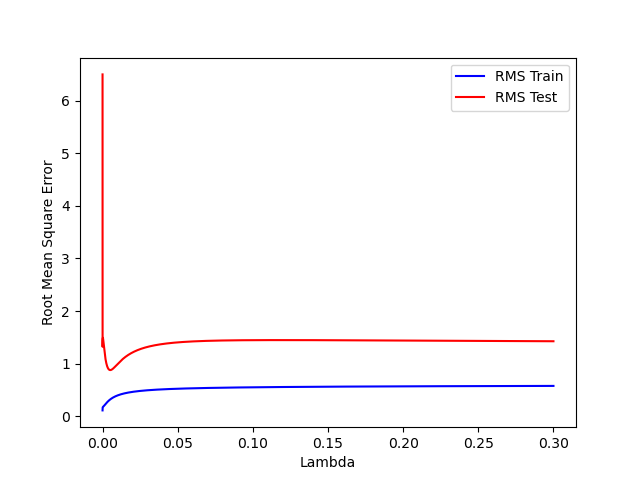
\includegraphics[scale=0.5]{img/Lambda_vs_RMS.png}
    \caption{Even with a slight increase in the regularization term $\lambda$, the RMS error on the testing set heavily decreases. }
    \label{fig:enter-label}
  \end{figure} 

\subsection{Least Squares Solution}

  Now that we have this form, we might as well just solve it. 

  \begin{theorem}[Least Squares Solution for Ridge Regression]
    The minimizer of the ridge loss is 
    \begin{equation}
      \hat{\beta} = (X^T X+ \lambda I)^{-1} X^T Y
    \end{equation}
  \end{theorem}
  \begin{proof}
    TBD
  \end{proof} 

  \begin{code}[MWS of Ridge Regression in scikit-learn]
    \noindent\begin{minipage}{.6\textwidth}
    \begin{lstlisting}[]{Code}
      import numpy as np 
      from sklearn.linear_model import Ridge  

      X = np.random.randn(10, 5) 
      y = np.random.randn(10)
      # regularization parameter
      model = Ridge(alpha=1.0)  
      model.fit(X, y) 
      print(model.score(X, y))  
      print(model.intercept_)
      print(model.coef_) 
      print(model.predict(np.array([[1, 2, 3, 4, 5]]))) 
    \end{lstlisting}
    \end{minipage}
    \hfill
    \begin{minipage}{.39\textwidth}
    \begin{lstlisting}[]{Output}
      0.8605535024325397
      -0.28291076492665157
      [-0.10400521 -0.7587073  -0.05116735  1.16236649 -0.0401323 ]
      [2.39097184]
      .
      .
      .
      .
      .
      .
    \end{lstlisting}
    \end{minipage}
  \end{code}

\subsection{Bias Variance Tradeoff}

  \begin{theorem}[Bias Variance Decomposition of Ridge Regression]
    TBD 
  \end{theorem}

  From a computational point of view, we can see that by adding the $\lambda I$ term, it \textit{dampens} the matrix so that it does become invertible (or well conditioned), allowing us to find a solution. The higher the $\lambda$ term, the higher the damping effect. 

\subsection{Concentration Bounds}

  The next theorem compares the performance of the best ridge regression estimator to the best linear predictor. 

  \begin{theorem}[Hsu, Kakade, Zhang, 2014 \cite{hsu2014random}] 
    Suppose that $||X_i|| \leq r$ and let $\beta^T x$ be the best linear approximation to $f(x)$. Then, with probability at least $1 - 4 e^{-t}$, we have
    \begin{equation}
      r(\hat{\beta}) - r(\beta) \leq \bigg( 1 + O \bigg( \frac{1 + r^2 / \lambda}{n} \bigg) \bigg) \frac{\lambda ||\beta||^2}{2} + \frac{\sigma^2}{n} \frac{\Tr(\Sigma)}{2 \lambda}
    \end{equation}
  \end{theorem}

  We can see that the $\lambda$ term exists in the numerator on $\frac{\lambda ||\beta||^2}{2}$ and in the denominator on $\frac{\Tr(\Sigma)}{2 \lambda}$. This is the bias variance tradeoff. The first term is the bias term, which is the penalty for not being able to fit the data as well. The second term is the variance term, which is the penalty for having a more complex model. So our optimal $\lambda$ in the theoretical sense would be the one that minimizes the sum of these two terms. In practice, it's not this clean since we have unknown quantities in the formula, but just like how we did cross validation over the model complexity, we can also do cross validation over the $\lambda$. The decomposition above just gives you a theoretical feeling of how these things trade off. 

\subsection{Tuning the Regularization Coefficient}
